%! TeX program = lualatex

\documentclass[11pt]{extarticle}

% Set 1-inch margins
\usepackage[margin=1in]{geometry}

% Set Times New Roman for text and Cambria Math for math fonts
\usepackage{fontspec}
\setmainfont{Times New Roman}

% Use Symbol font for non-alphabetic characters
\usepackage{textcomp}

% Set line spacing to single (no less than single-spacing)
\usepackage{setspace}
\setstretch{1.0}

% Package for handling citations
\usepackage[backend=biber,style=numeric,sorting=none]{biblatex}
\addbibresource{references.bib}

% For inserting images and subcaptions
\usepackage{graphicx,subcaption} 
\usepackage{wrapfig}
\usepackage{svg}

% Begin document
\begin{document}

\textbf{Introduction:} Category theory is slowly beginning to permeate various ``applied'' disciplines by providing a unique framing of knowledge discovery processes to provide insight into how these processes can be composed together to yield novel knowledge generation. % TEJA: Ask if this topical sentence is stronger now
To explain the significance of this, the idea of compositionality is the characteristic that ``describes and quantifies how complex things can be assembled out of simple parts'' [1] and is a concept ubiquitous across mathematics but is seen acutely in the fundamentals of category theory.
The field of category theory studies, simply put, the "relationships that exist between things" which gives one a vantage point to think not on the minutiae of a particular problem but more broadly about how things in a problem space may ``fit together'' (i.e. ``be composed'').
By thinking at this level of abstraction, it can be observed broadly that a task common to nearly all disciplines is ``knowledge discovery'', the process of scrutinizing available data to generate novel insight about a particular field or topic. % TEJA: Does this seem natural?

\begin{wrapfigure}{r}{0.3\textwidth}
\centering
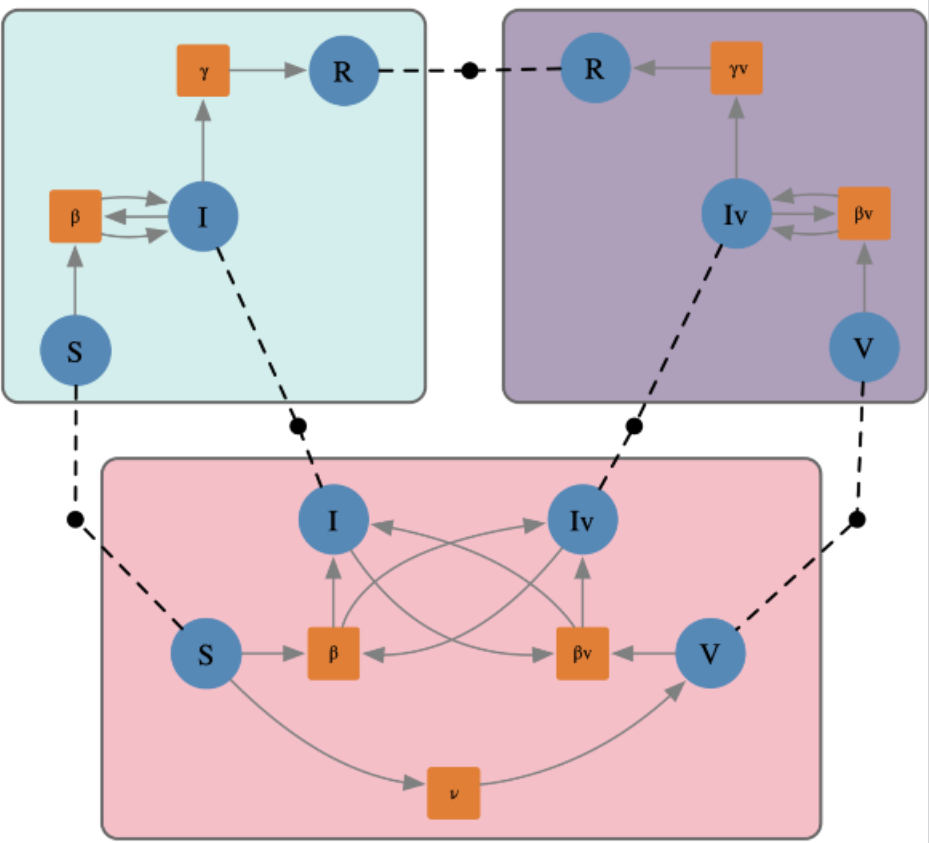
\includegraphics[width=0.3\textwidth]{sub_models}
\vspace{-10pt}
\caption{
  3 discovery processes (the three different petri nets in boxes) with relationships defined by arrows and lines inside of and between processes. % TEJA: How does caption read?
}
\vspace{30pt}
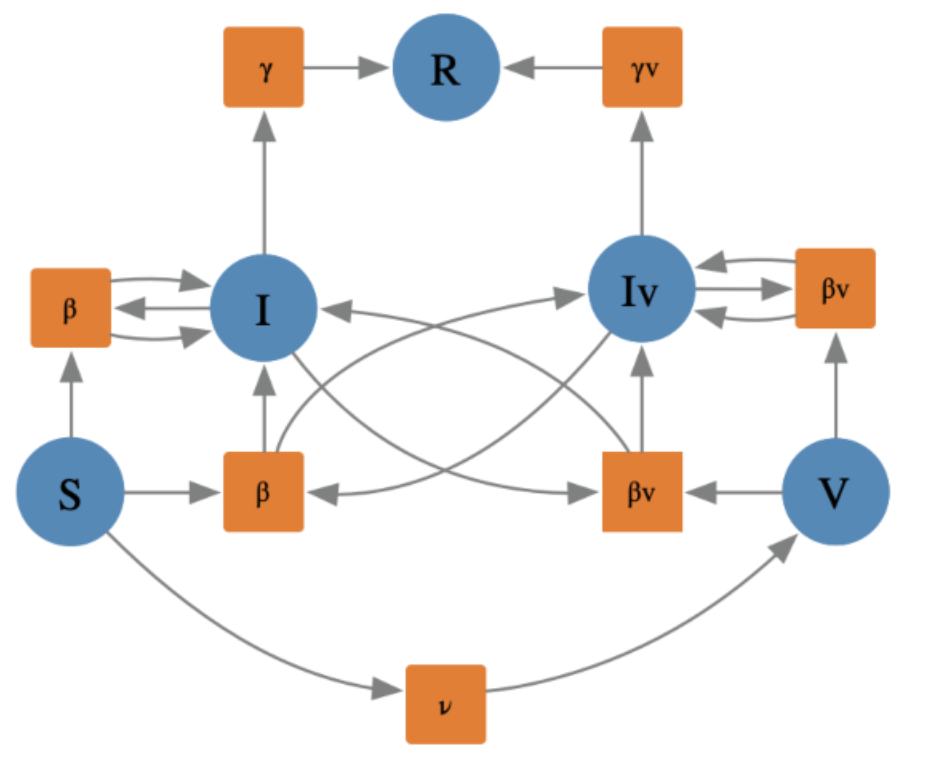
\includegraphics[width=0.25\textwidth]{composed_model}
\vspace{-10pt}
\caption{
  Composition of the 3 discovery processes into one novel discovery process. % TEJA: How does caption read?
}
\end{wrapfigure}

Motivating the objectives of this proposal is my experience within Georgia Tech Research Institute and the US Centers for Disease Control where I noticed that knowledge discovery processes can appear similar across disciplines but due to domain specifics, adapting old discovery methods to novel applications can be a laborious and time consuming process. 
To give a concrete example of this, consider figure 1 which depicts 3 different dynamical systems (denoted by the different figures within each colored box) given by petri nets, a diagrammatic language well-understood in the terms of category theory. % TODO: Add citations for petri nets
Within each box, the petri nets are modeling variations of the SIR compartmental model to drive knowledge discovery in epidemiology (compartmental models are widespread across epidemiology but have application in economics, ecology, and beyond). 
Here, circles represent populations (S for susceptible, I for infected, R for recovered, V for vaccinated, and Iv for infected-vaccinated), squares represent variables that attenuate the strength of relationships, given by arrows, are between populations, and dotted lines relate populations across the three knowledge discovery processes.
Figure 2 then shows the result of how composing these models across dotted lines can reuse separate knowledge discovery processes while also simplifying them into one novel knowledge discovery process subsuming former knowledge discovery efforts.
\textbf{It is the goal of this proposal to demonstrate how a category theoretic treatment of knowledge discovery can improve the fundamental understanding of relationships between discovery processes, reduce the time needed to find relationships, and how processes can be resused to gain insight into novel applications.}

\textbf{Research Plan:} I will dedicate my PhD studies at Harvard University to investigate the promise of applying category theory in knowledge discovery under the advisement of Professor Nathaniel Osgood.
Additionally, I will continue to maintain a strong collaboration relationship with the Topos Institute and the GATAS Lab at the University of Florida who are pioneering applied category theory approaches and technology.
In the course of this work, I will pursue the following objectives:

\textbf{Objective 1: Map the Knowledge Discovery Process To Category Theoretic Language.} To drive exploration of the general knowledge discovery process, I will pick three heterogeneous data sets that vary by how they are sampled over time and by what kind of data they contain. 
Then, I will construct general knowledge discovery pipelines to scrutinize these data sets through various data science techniques (such as clustering or prediction methods) to simulate deriving novel insights data in general.
After creating these pipelines, I will then explore manually how these data sets could be related to one another.

Once several relationships that could exist within and between data sets have been enumerated, I will then proceed to map these knowledge discovery processes on to various categorical structures.
First, I will use $\mathscr{C}$-sets, which describes a functor mapping a schema category $\mathscr{C}$ into the category $\mathbb{Set}$ (as objects) and functions between them (as morphisms) [@osgood] % TODO: Add a sentence after this about what this is exactly
Then, to assess how reasonable the identified relationships are, I will use a decorated copresheaf structure (known as "acsets") to compute a presentation of the schema represented by the acset. [@lynch]
This objective will be completed when I have created an adequate $C$-set presentation that, to the best of my ability, describes the relationships present within and between these datasets.

% The data I will use comprises of the following: [IPUMS](http://ipums.org/) census microdata for a variety of different demographic information across the globe and a ton for the USA, [ERA5](https://cds.climate.copernicus.eu/cdsapp#!/dataset/reanalysis-era5-single-levels?tab=overview) & [National Centers for Environmental Information](https://www.ncei.noaa.gov) These two datasets have such a wide array of climate related data for the entire globe on a fantastic time resolution, and [Pharmetrics Plus](https://www.iqvia.com/locations/united-states/library/fact-sheets/iqvia-pharmetrics-plus) a 35+ million USA patient database of patient medical records from across the entire country.
% What motivates this particular selection of data sets is the significant differences between them: the IPUMS data is regularly sampled across the US at a state or coarse population level at regular and monthly time intervals, the ERA5 and NCEI data is also regularly sampled but at a much more granular time and temporal resolution, and the patient data set varies significantly by geospatial region as well as having extremely irregular or even random sampling intervals for patient encounters.

\textbf{Objective 2: Prototype Knowledge Discovery for a Specific Topic Using Category Theoretic Framing.} At this stage, the data sets I have been exploring have been framed using the language of category theory.
Now, I will take this framing of these data sets to drive novel knowledge discovery for a particular topic beyond what is generally possible with data science approaches.
I will explore what methods are possible to compute on top of this data now taking inspiration from previous work done by Osgood and Zardini. % TODO: Add citation from An Algebraic Framework for Structured Epidemic Modeling for Nate. Maybe cut Zardini? 
Additionally, I will identify what questions are possible to be answered in this new framework beyond what could be addressed during objective 1.
Objective 2 will be completed once I have not only determined what sorts of methods would be most salient to compute upon this framing but have also uncovered and attempted to address novel questions that could only be asked by using a categorical framing.

\textbf{Objective 3: Explore Composition of Knowledge Discovery Processes.} At this stage, I will rexamine objectives 1 and 2 with another set of data or, at least, a different $C$-set presentation to frame another knowledge discovery pipeline in the language of category theory.
Once this secondary knowledge discovery pipeline has been framed using category theoretic language, I am now at one of the most exciting points of this work: exploring how these knowledge discovery pipelines can be composed with one another.
An example of this idea given in Figure a and Figure b.
Using petri nets, a convenient diagrammatic language that has a well-described category theoretic treatment, one can describe knowledge discovery processes as separate diagrams (as shown in Figure a) and then explore how these diagrams could potentially compose.
Then, in Figure b, a final diagram incorporating all knowledge discovery processes could be created that is itself a novel knowledge discovery process that can drive insight across different knowledge discovery pipelines.


\textbf{Intellectual Merit:} This project aims to advance approaches in knowledge discovery by leveraging category theory formalizations to observe novel relationships present between knowledge products. 
The use of category theory to harmonize heterogeneous datasets across knowledge discovery processes could offer a new perspective in how traditional discovery could be applied on top of data scaffolded in a category theory framing.
Additionally, by taking advantage of this framing, prior knowledge discovery pipelines could be reused and combined into novel pipelines to address changing needs in engineering or other applied contexts. 

\textbf{Broader Impacts:} By viewing knowledge discovery processes as compositional objects, this could revolutionize how complex systems are analyzed across various disciplines.
Furthermore, as the limits of applied category theoretic machinery is explored in the course of this work, new frontiers in applied category theory could be explored.
This could inform the foundational mathematics undergirding any applications while also leading to the creation of computational software based on these insights.
Finally, this framing could improve the construction of knowledge discovery processes from the beginning by allowing one to easily reason about how a given process in development could be composed in the future or with other pipelines while in development.
This way of framing problems is beginning to permeate specific domains such as engineering system design [2], database architecture [3], and machine learning [4]. % TODO: Incorporate this here somehow

\textbf{References:} [1] \textit{Compositionality}, 2024. [2] \textit{ACT4ED}, MIT 1.S980 [3] \textit{Algebraic Databases}, Shultz, et. al., 2016. [4] \textit{Category theory in machine learning}, Gavranović, 2021. [5] \textit{Measuring the impact of knowledge loss: a longitudinal study} Massingham [6] \textit{Emergency Preparedness for Vulnerable Populations}, Nick [7] \textit{An Algebraic Framework for Structured Epidemic Modelling.}, Libkind, et. al., 2022. 


\end{document}
